%\documentstyle[epsf,twocolumn]{jarticle}       %LaTeX2.09仕様
%\documentclass[twocolumn]{jarticle}     %pLaTeX2e仕様
\documentclass{jarticle}     %pLaTeX2e仕様

%一枚組だったら[twocolumn]関係のとこ消す

\setlength{\topmargin}{-45pt}
%\setlength{\oddsidemargin}{0cm} 
\setlength{\oddsidemargin}{-7.5mm}
%\setlength{\evensidemargin}{0cm} 
\setlength{\textheight}{24.1cm}
%setlength{\textheight}{25cm} 
\setlength{\textwidth}{17.4cm}
%\setlength{\textwidth}{172mm} 
\setlength{\columnsep}{11mm}

\kanjiskip=.07zw plus.5pt minus.5pt

\usepackage[dvipdfm]{graphicx}
\usepackage{ccaption}
\usepackage{algorithm}
\usepackage{algorithmic}
\usepackage{subcaption}
\usepackage{enumerate}
\usepackage{comment}
\usepackage{url}
\usepackage{multirow}
\usepackage{diagbox}
\usepackage{amssymb}
\usepackage{mathtools}
\usepackage{wrapfig}
\usepackage{graphicx}
\usepackage{float}
\usepackage{amsmath}
\usepackage{lipsum}


\begin{document}
  \noindent
  \hspace{1em}

  \today Creation班 ゼミ
  \hfill
  \ \  西村昭賢 

  \vspace{2mm}
  \hrule
  \begin{center}
  {\Large \bf 進捗報告}
  \end{center}
  \hrule
  \vspace{3mm}


\section{やったこと}
\begin{itemize}
  \item 突然変異関数の見直し
  \item 世代数を増やして数値実験
\end{itemize}


\section{突然変異関数の見直し}
以前は, 突然変異率を基に個体群から突然変異させる個体を選び, 選ばれた個体については遺伝子座をランダムに 1 つ選択しその遺伝子座について要素を変更する操作だった. \par
初期収束が起こりやすそうだったため見直しを検討し, 突然変異率を各遺伝子座に適用して要素を変更する操作に変更した.



\section{世代数を増やして数値実験}
多目的 GA に関して解が収束しきっていないようだったため, 世代数を増やし上記の突然変異を適用した.


\begin{table}[ht]
  \centering
  \caption{GAのパラメータ (変更部分を記載)}
  \vspace{-0.3cm}
  \label{table:gaparam}
  \scalebox{1.0}[1.0]{
    \begin{tabular}{|c|c|}
      \hline
      パラメータ名 & 値 \\ \hline \hline
      世代数 & 50 ⇒ \textbf{100} \\ \hline     
      個体数 & 50     \\ \hline
      遺伝子長 & 調整するカードの種類数 $\times$ 3       \\ \hline
      交叉率 & 0.4 ⇒ \textbf{0.6} \\ \hline
      交叉の種類 & 2 点交叉 \\ \hline
      突然変異率 & 0.2 ⇒ \textbf{1/遺伝子長} \\ \hline
      選択 & 1 個体だけエリート保存, その他はトーナメント方式 \\ \hline
      トーナメントサイズ &  3 \\ \hline
      \end{tabular}
  }
  \end{table}

\subsection{結果}
先行研究で用いられていたデッキ間の勝率に関する目的関数とデッキ内のパラメータの総変更量に関する目的関数の 2 目的の GA に関して, 卒業研究のデータと比較した.
図 \ref{fig:fwfp}, \ref{fig:fwfc} に結果を示す. 図の赤点が卒業研究のデータ, 黒点が今回の実験のデータである.
パラメータの変更や突然変異の見直しにより, 良好なパレートフロントが得られた. 

\begin{figure}[ht]
  \centering
  \includegraphics[width=120mm]{assets/fwfp.eps}
  \vspace{-0.3cm}
  \caption{最終世代のパレートフロント (縦軸が勝率, 横軸がパラメータの変化量)}
  \label{fig:fwfp}
\end{figure}

\begin{figure}[ht]
  \centering
  \includegraphics[width=120mm]{assets/fwfc.eps}
  \vspace{-0.3cm}
  \caption{最終世代のパレートフロント (縦軸が勝率, 横軸が調整されたカードの枚数)}
  \label{fig:fwfc}
\end{figure}

また,多目的 GA として 3 目的 GA も表 \ref{table:gaparam} のパラメータで実験し結果をまとめた .
図 \ref{fig:fwfc_reall}, \ref{fig:fwfp_reall} において, 赤点が 2 目的 GA, 黒点が 3 目的GA, 緑点が卒業研究で用いた単目的 GA, 青点が卒業研究における提案手法のデータである. 
単目的 GA に関しては 表 \ref{table:gaparam} のパラメータで再実験していない.

\begin{figure}[ht]
  \centering
  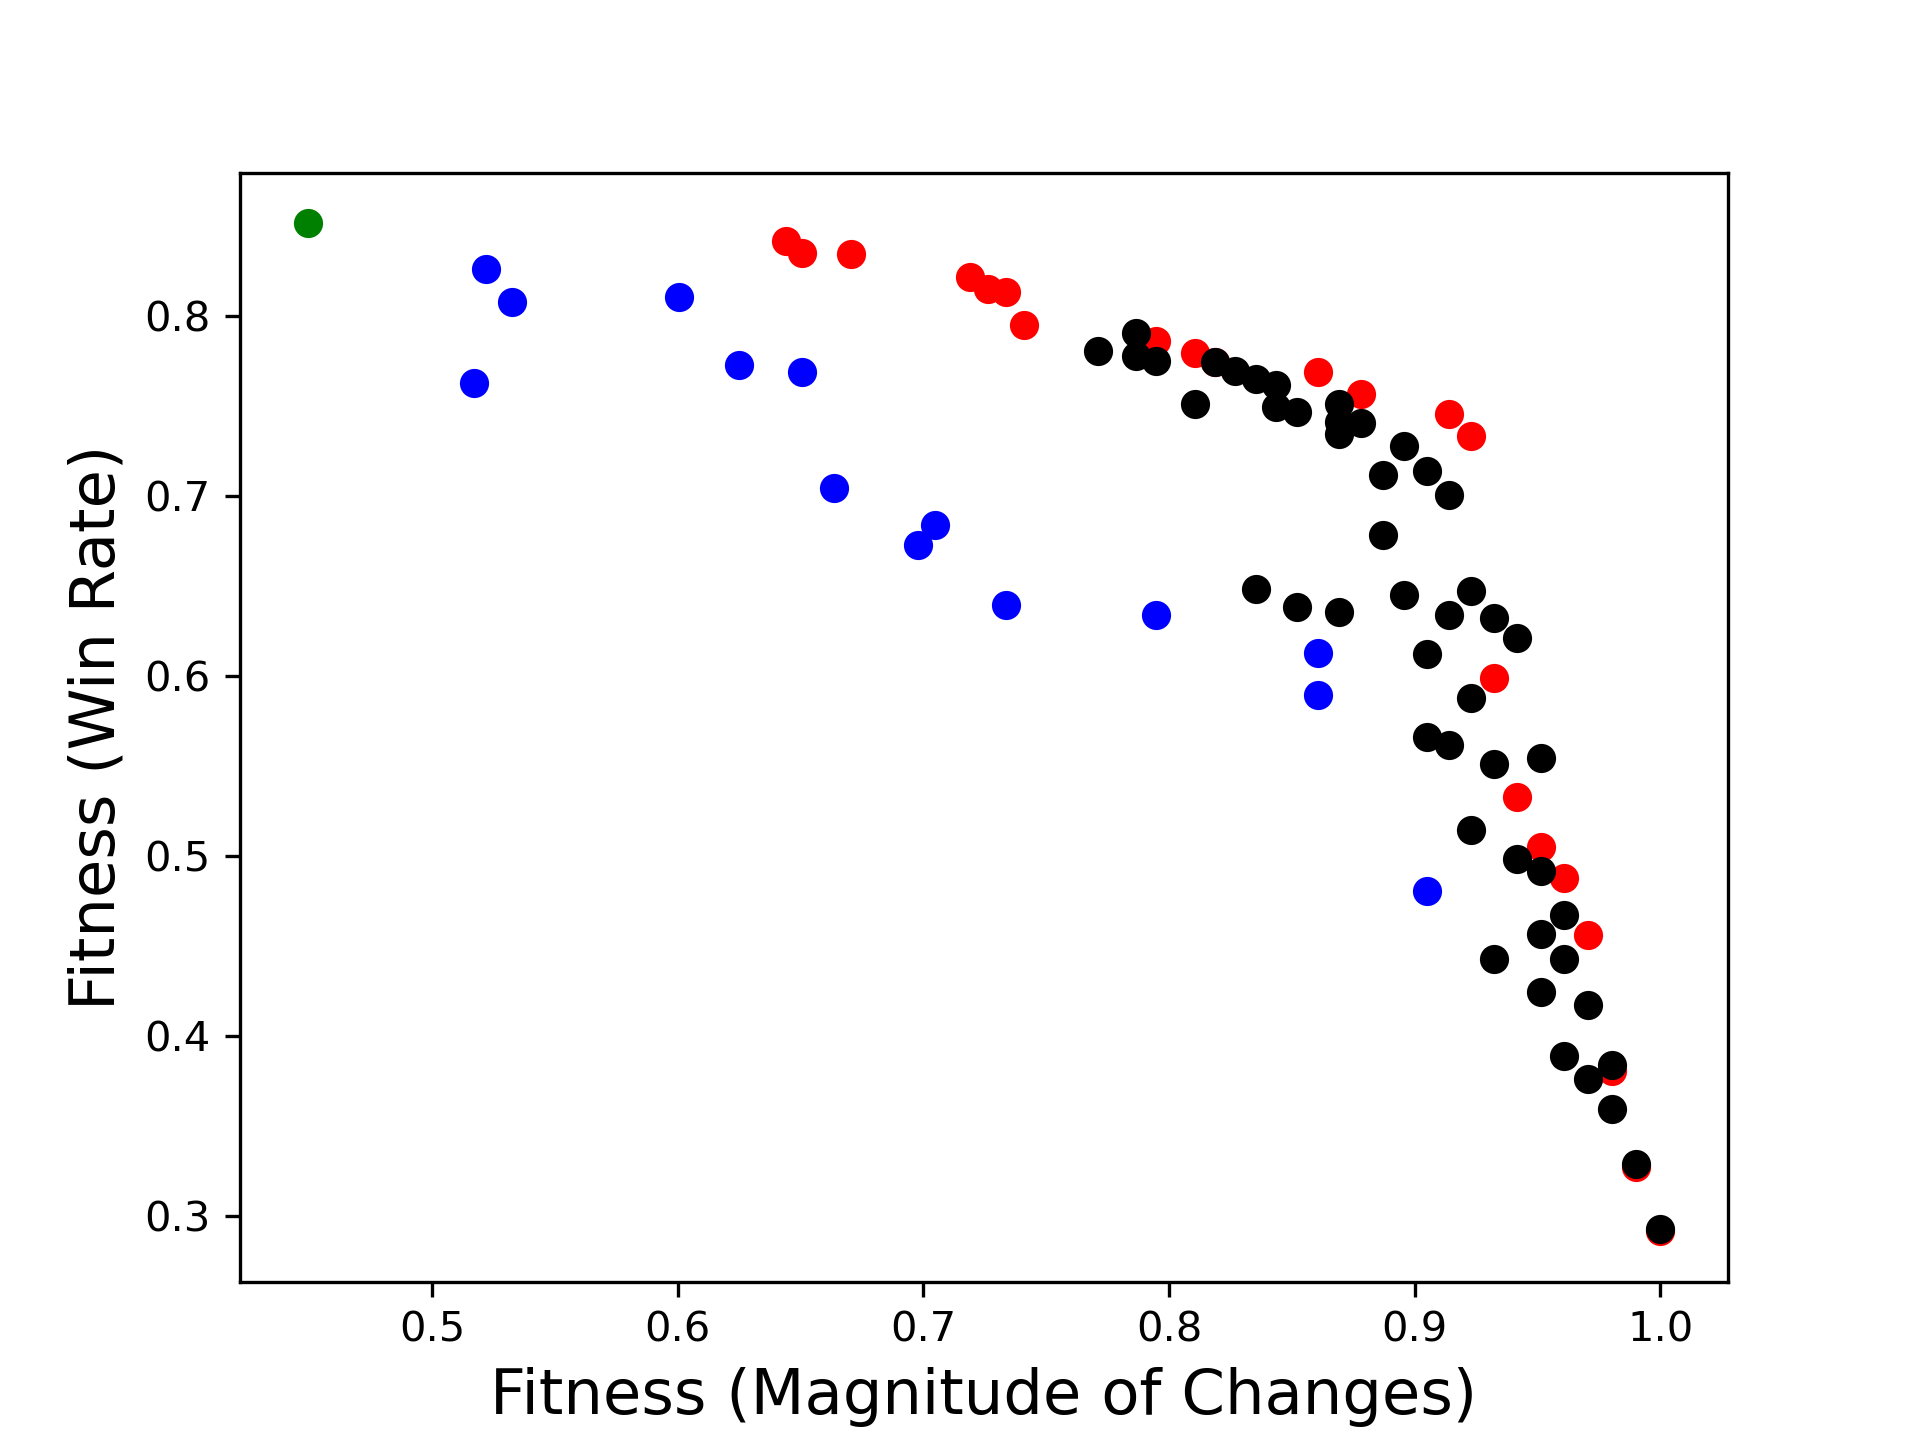
\includegraphics[width=120mm]{assets/fwfp_reall.eps}
  \vspace{-0.3cm}
  \caption{各手法の最終世代における最も良好な解, パレートフロント (縦軸が勝率, 横軸がパラメータの変化量)}
  \label{fig:fwfp_reall}
\end{figure}

\begin{figure}[ht]
  \centering
  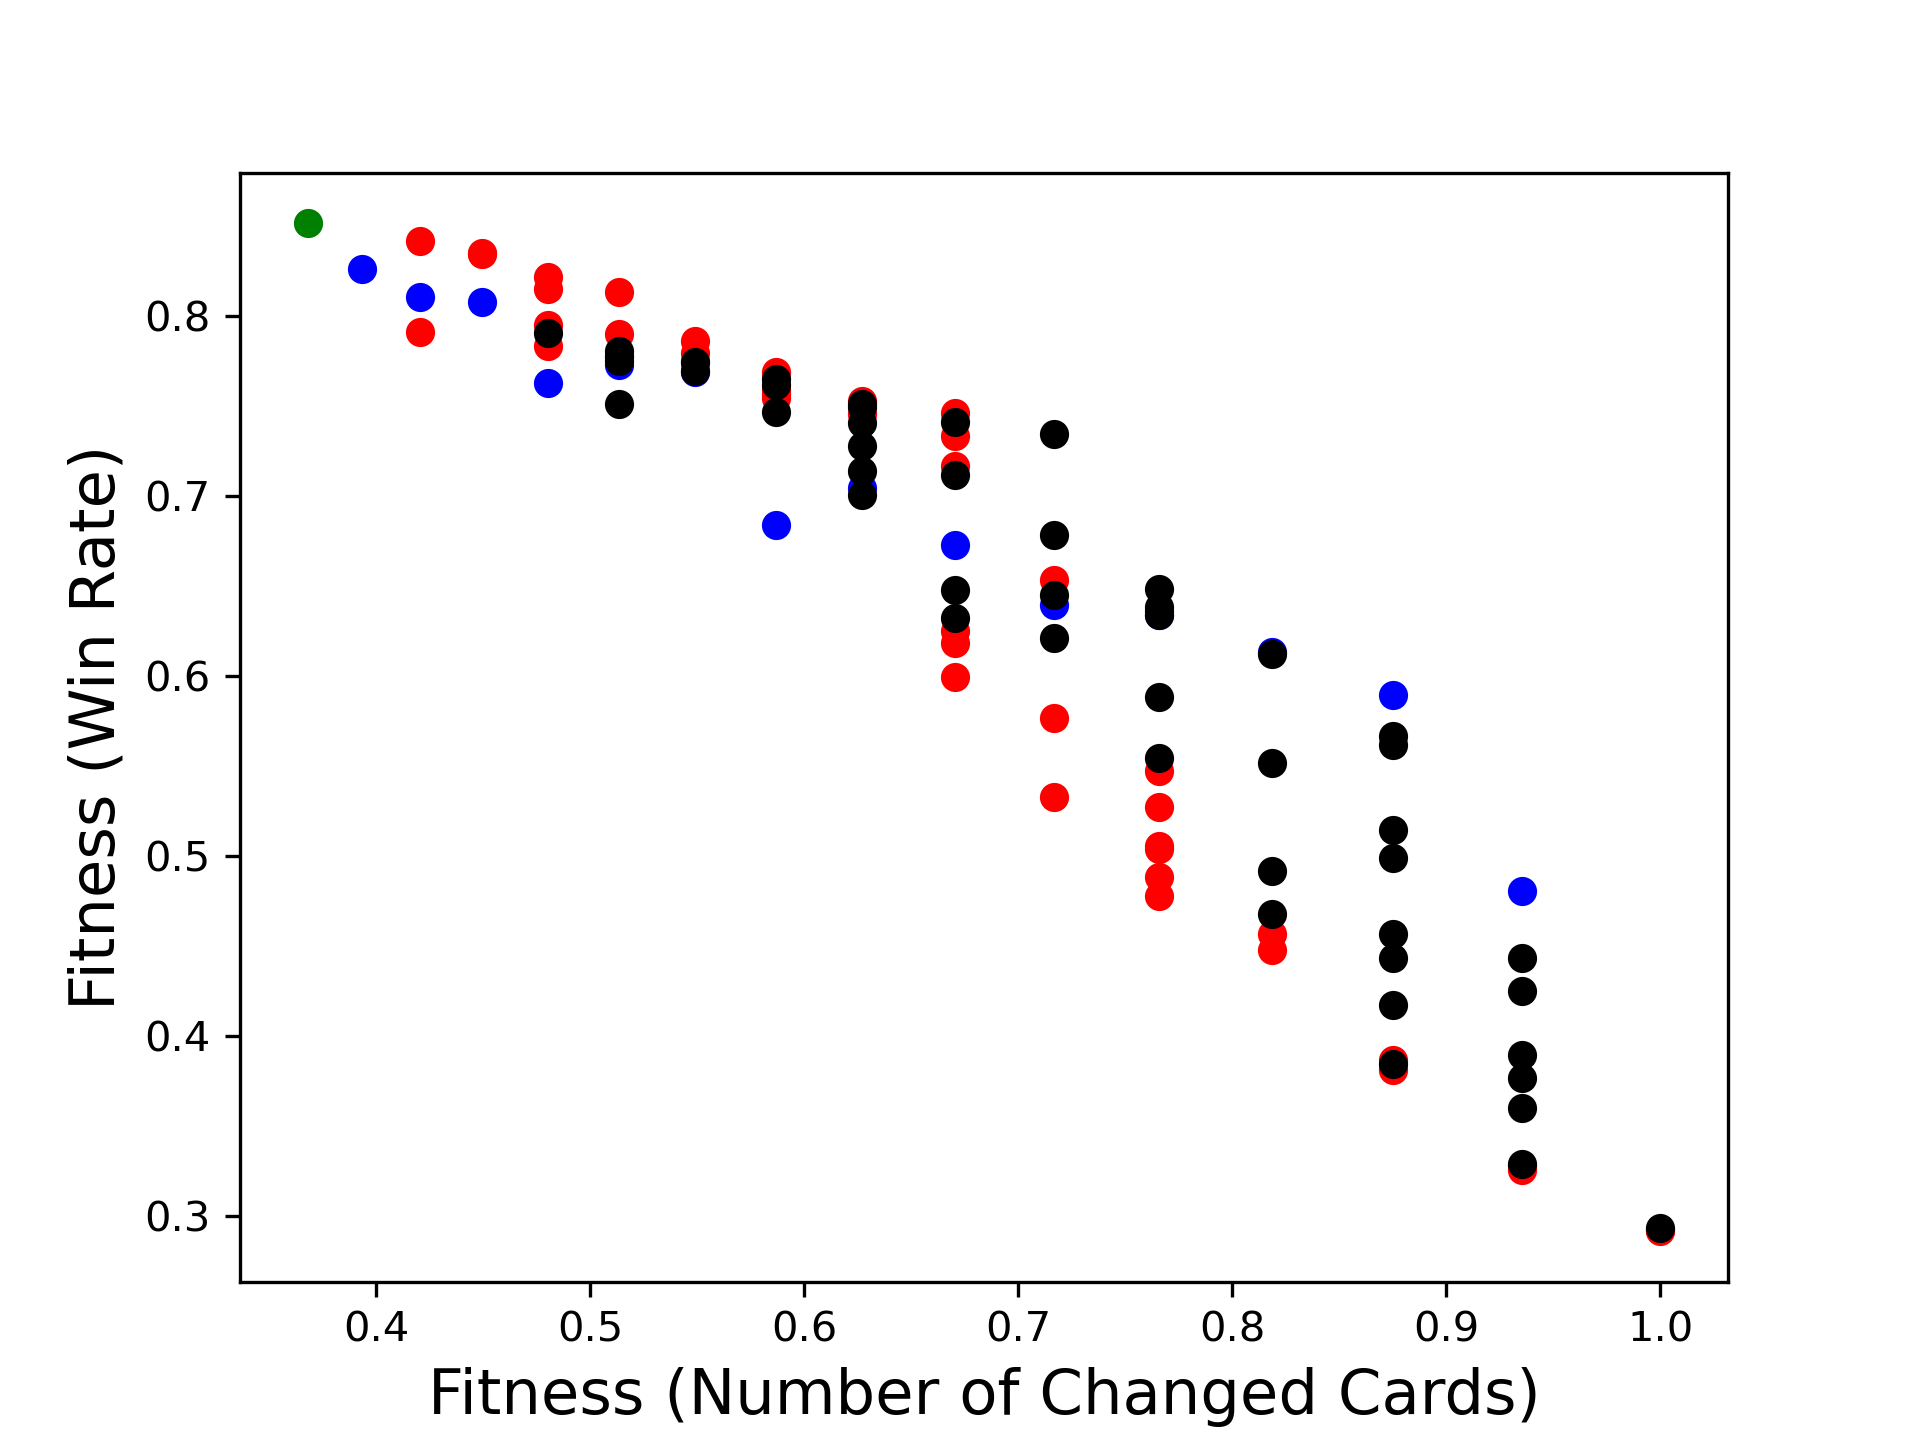
\includegraphics[width=120mm]{assets/fwfc_reall.eps}
  \vspace{-0.3cm}
  \caption{各手法の最終世代における最も良好な解, パレートフロント (縦軸が勝率, 横軸が調整されたカードの枚数)}
  \label{fig:fwfc_reall}
\end{figure}



\section{今後の方針}
\begin{itemize}
  \item 勝率と調整されるカードの枚数の 2 目的で GA
  \item Optuna のパラメータチューニング
\end{itemize}

%index.bibはtexファイルと同階層に置く
%ちゃんと\citeしないと表示されない(1敗)
\bibliography{index.bib}
\bibliographystyle{junsrt}

\end{document}